% ===================================================================
% Arquivo: capitulos/parte-III-pilares/cap-10-perda-binaria.tex
% ===================================================================

\chapter{Funções de Perda para Regressão}
\label{cap:perda-regressao}

Até agora foi visto o funcionamento da retropropagação, e como ela faz uso dos otimizadores, os quais funcionam como um barco, percorrendo a função de perda em busca de pontos de mínimos. Além disso, em seguida foram vistas diversas funções de ativação, começando pelas sigmoidais, depois pelas retificadoras, e por fim uma coletânea de diferentes funções. Contudo, está na hora de entender o outro lado da retropropagação: as funções de perda.

Para isso, esse capítulo busca explicar diversas funções de perda e suas aplicações, começando pelas funções para problemas de regressão, conhecendo as clássicas erro quadrático médio e erro absoluto médio, além da \textit{hubber loss}, uma função que busca unir o melhor dessas duas funções de perda. Seguindo adiante, são introduzidas as funções de perda para classificação binária, como a \textit{BCE}. Visto os problemas de classificação binária, é possível também conhecer os problemas de classifação multi com a \textit{categorical cross entropy}.

Mais adiante, está apresentado não funções, mas esquemas de como a perda pode ser medida para problemas como o de redes adversárias. Mas as perdas não são a única forma de medir como um modelo está performando, para isso, o final do capítulo é dedicado para explicar outros diferentes métodos de medir o desempenho do modelo que está sendo construído.

\section{A Intuição da Perda: Medindo o Erro do Modelo}

\section{Exemplo Ilustrativo: Jogando Dados}

\section{Funções de Perda para Regressão para Propósitos Gerais}

\subsection{Erro Quadrático Médio (Mean Squared Error - MSE)}


\begin{equacaodestaque}{Erro Quadrático Médio (MSE)}
    L_{\text{MSE}} = \frac{1}{N} \sum_{i=1}^{N} (y_i - \hat{y}_i)^2
    \label{eq:mse}
\end{equacaodestaque}

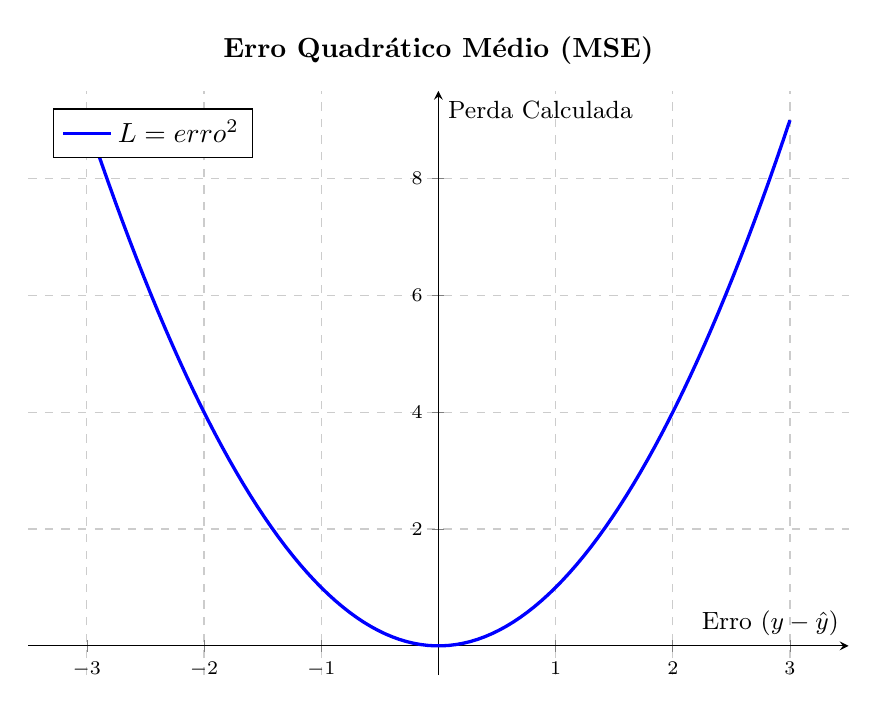
\begin{tikzpicture}
    \begin{axis}[
        title={Erro Quadrático Médio (MSE)},
        xlabel={Erro ($y - \hat{y}$)},
        ylabel={Perda Calculada},
        axis lines=middle,          % Eixos centrados em (0,0)
        grid=major,                 % Adiciona uma grade principal
        grid style={dashed, gray!40}, % Estilo da grade
        xmin=-3.5, xmax=3.5,        % Limites do eixo x
        ymin=-0.5, ymax=9.5,         % Limites do eixo y
        legend pos=north west,      % Posição da legenda
        width=12cm,                 % Largura do gráfico
        height=9cm,                 % Altura do gráfico
        title style={font=\bfseries},
        label style={font=\small},
        tick label style={font=\scriptsize}
    ]
        % Adiciona o gráfico da função x^2
        \addplot[
            domain=-3:3, 
            samples=100, 
            color=blue, 
            very thick
        ] {x^2};
        
        % Adiciona uma entrada na legenda
        \addlegendentry{$L = \text{erro}^2$}
    \end{axis}
\end{tikzpicture}

\begin{equacaodestaque}{Derivada do MSE}
    \frac{\partial L_{\text{MSE}}}{\partial \hat{y}_i} = \frac{2}{N}(\hat{y}_i - y_i)
    \label{eq:mse-derivada}
\end{equacaodestaque}


\subsection{Erro Absoluto Médio (Mean Absolute Error - MAE)}


\begin{equacaodestaque}{Erro Absoluto Médio (MAE)}
    L_{\text{MAE}} = \frac{1}{N} \sum_{i=1}^{N} |y_i - \hat{y}_i|
    \label{eq:mae}
\end{equacaodestaque}

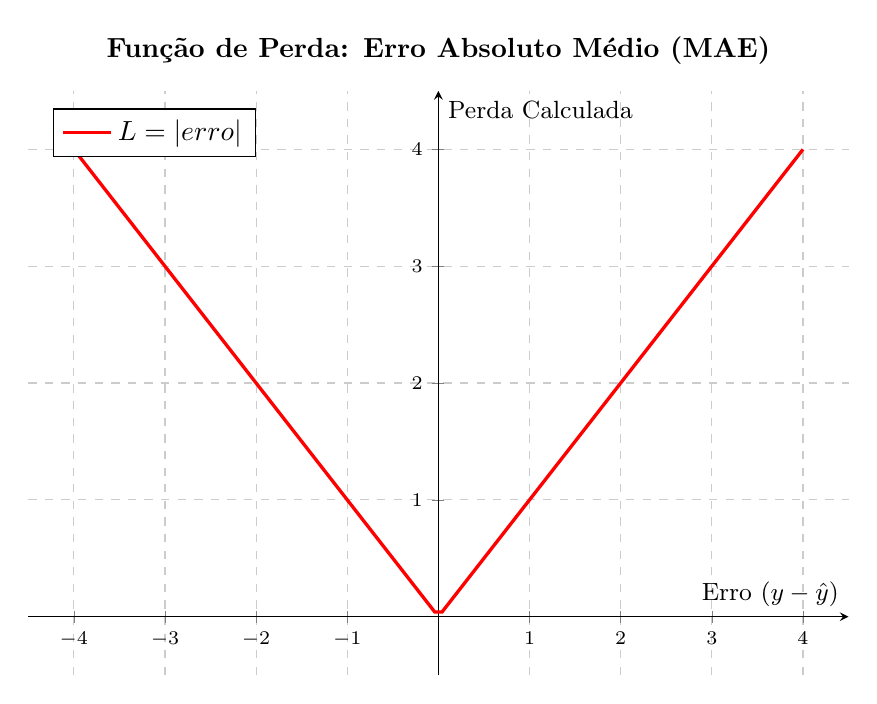
\begin{tikzpicture}
    \begin{axis}[
        title={Função de Perda: Erro Absoluto Médio (MAE)},
        xlabel={Erro ($y - \hat{y}$)},
        ylabel={Perda Calculada},
        axis lines=middle,          % Eixos centrados em (0,0)
        grid=major,                 % Adiciona uma grade principal
        grid style={dashed, gray!40}, % Estilo da grade
        xmin=-4.5, xmax=4.5,        % Limites do eixo x
        ymin=-0.5, ymax=4.5,         % Limites do eixo y
        legend pos=north west,      % Posição da legenda
        width=12cm,                 % Largura do gráfico
        height=9cm,                 % Altura do gráfico
        title style={font=\bfseries},
        label style={font=\small},
        tick label style={font=\scriptsize}
    ]
        % Adiciona o gráfico da função abs(x)
        \addplot[
            domain=-4:4, 
            samples=100, 
            color=red, 
            very thick
        ] {abs(x)};
        
        % Adiciona uma entrada na legenda
        \addlegendentry{$L = |\text{erro}|$}
    \end{axis}
\end{tikzpicture}

\begin{equacaodestaque}{Derivada do MAE}
    \frac{\partial L_{\text{MAE}}}{\partial \hat{y}_i} = \frac{1}{N} \cdot \text{sgn}(\hat{y}_i - y_i) = 
    \begin{cases} 
      +\frac{1}{N} & \text{se } \hat{y}_i > y_i \\
      -\frac{1}{N} & \text{se } \hat{y}_i < y_i \\
      0 & \text{se } \hat{y}_i = y_i
    \end{cases}
    \label{eq:mae-derivada}
\end{equacaodestaque}


\subsection{Huber Loss: O Melhor de Dois Mundos}


\begin{equacaodestaque}{Huber Loss}
    L_{\delta}(y, \hat{y}) = 
    \begin{cases} 
      \frac{1}{2}(y - \hat{y})^2 & \text{para } |y - \hat{y}| \le \delta \\
      \delta (|y - \hat{y}| - \frac{1}{2}\delta) & \text{caso contrário}
    \end{cases}
    \label{eq:huber-loss}
\end{equacaodestaque}

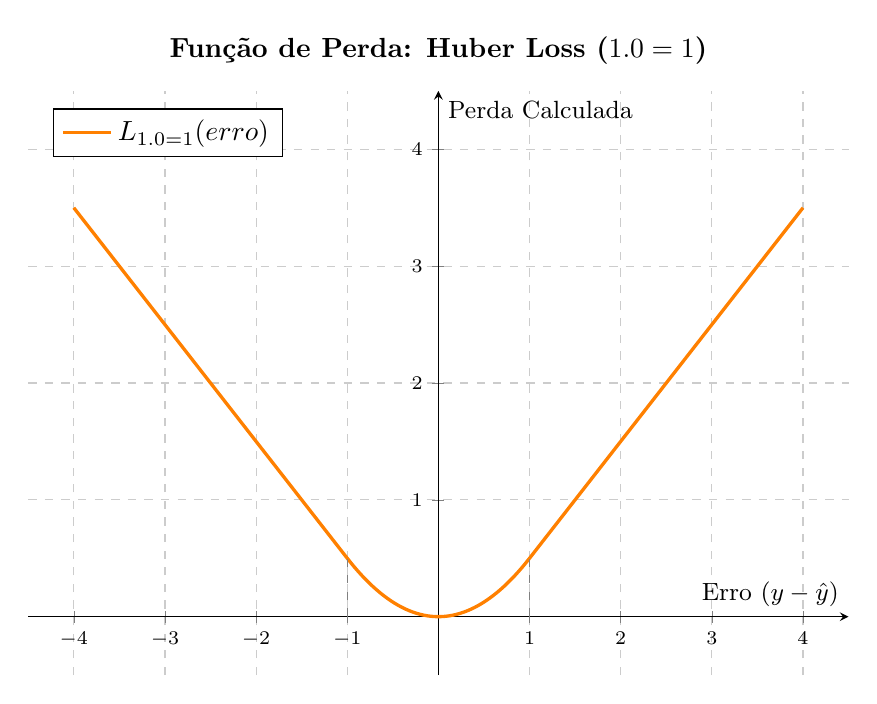
\begin{tikzpicture}
    \begin{axis}[
        title={Função de Perda: Huber Loss ($\delta=1$)},
        xlabel={Erro ($y - \hat{y}$)},
        ylabel={Perda Calculada},
        axis lines=middle,          % Eixos centrados em (0,0)
        grid=major,                 % Adiciona uma grade principal
        grid style={dashed, gray!40}, % Estilo da grade
        xmin=-4.5, xmax=4.5,        % Limites do eixo x
        ymin=-0.5, ymax=4.5,         % Limites do eixo y
        legend pos=north west,      % Posição da legenda
        width=12cm,                 % Largura do gráfico
        height=9cm,                 % Altura do gráfico
        title style={font=\bfseries},
        label style={font=\small},
        tick label style={font=\scriptsize}
    ]
        % Define o valor de delta
        \def\delta{1.0}

        % Adiciona o gráfico da função Huber usando uma expressão condicional
        % Se |x| <= delta, usa 0.5*x^2. Senão, usa delta*(|x| - 0.5*delta).
        \addplot[
            domain=-4:4, 
            samples=201, % Samples ímpares para incluir o ponto x=0
            color=orange, 
            very thick
        ] { abs(x) <= \delta ? 0.5*x^2 : \delta*(abs(x) - 0.5*\delta) };
        
        % Adiciona uma entrada na legenda
        \addlegendentry{$L_{\delta=1}(\text{erro})$}

        % Opcional: Adiciona linhas para mostrar a transição em delta
        \draw[dashed, gray] (axis cs:-\delta, 0) -- (axis cs:-\delta, {\delta*(\delta-0.5*\delta)});
        \draw[dashed, gray] (axis cs:\delta, 0) -- (axis cs:\delta, {\delta*(\delta-0.5*\delta)});

    \end{axis}
\end{tikzpicture}

\begin{equacaodestaque}{Derivada da Huber Loss}
    \frac{\partial L_{\delta}}{\partial \hat{y}} = 
    \begin{cases} 
      \hat{y} - y & \text{para } |\hat{y} - y| \le \delta \\
      \delta \cdot \text{sgn}(\hat{y} - y) & \text{caso contrário}
    \end{cases}
    \label{eq:huber-loss-derivada}
\end{equacaodestaque}

\subsection{Perda Log-Cosh}

\section{Lidando com a Escala: Foco no Erro Relativo}

\subsection{Erro Quadrático Médio Logarítmico (MSLE)}

\section{Mudando o Objetivo da Previsão: Além da Média}

\subsection{Perda Quantílica}

\subsection{Perda Epsilon-Insensível}

\section{Perdas Baseadas em Distribuições de Dados}

\subsection{Perda de Poisson}

\subsection{Perda de Tweedie}

\subsection{Divergência Kullback-Leibler}

\section{Comparativo: Funções de Perda para Regressão}

\section{Fluxograma: Escolhendo a Função de Perda Ideal}